%\documentclass[conf]{new-aiaa}
\documentclass[journal]{new-aiaa} %for journal papers
\usepackage[utf8]{inputenc} % Used by Colin
\usepackage{xcolor} % Used by Colin
\usepackage{soul} % Used by Colin

\usepackage{graphicx} % Used by Colin
\usepackage{amsmath} % Used by Colin
\usepackage[version=4]{mhchem} % Used by Colin
\usepackage{siunitx} % Used by Colin
\usepackage{longtable,tabularx} % Used by Colin
\setlength\LTleft{0pt} % Used by Colin

% Custom packages
\usepackage{subcaption} % Used by Colin
\usepackage{makecell}
\usepackage{comment}

% Packages to allow InkScape Text to Display and Autoformat in figures
\graphicspath{{Photos/}{Photos/MUFASA/}{Photos/CFD/}{Photos/CFD/Coefficients}{Photos/Results/ModelVerification/}{Photos/Stability/}{Photos/Aircraft/}{Photos/Results/HandlingQualities/}{Photos/Results/ResponseQualities/}} % The subfolders where images are stored

\usepackage{multirow} % Allows for multirow table entries
\usepackage{array} % Allows for centered table entries
\usepackage{booktabs} % Allows for centered table entries
\usepackage{threeparttable} % Aligns table caption to be the width of the table

\newcommand{\pbox}[1]{\boxed{\phantom{#1}}} % Creates phantom (ie. empty) boxes in equations

\title{Writing Tips for the AERO-CORE Lab} %Title to be <= 12 words as per: https://www.aiaa.org/publications/journals/Journal-Author#follow-the-minimum-formatting-requirements

\author{
	Benjamin Durante\footnote{MSc, Department of Mechanical and Manufacturing Engineering}
}
\affil{University of Calgary, Calgary, Alberta, Canada, T2N 4V8}

\begin{document}

\newcommand{\MufasaLength}{1.30}
\newcommand{\MufasaWidth}{0.96}
\newcommand{\MufasaWeight}{51.6}
\newcommand{\MAC}{c_{\textup{mean}}}
\newcommand{\MACone}{c_{\textup{mean}_{1}}}
\newcommand{\MACtwo}{c_{\textup{mean}_{2}}} % Document containing variables used throughout

	\maketitle
	% PURPOSE: Each full-length paper must have a summary-type abstract of 100 to 200 (maximum) words in one paragraph, without numerical references, acronyms, or abbreviations. The abstract indicates the subjects dealt with in the paper and states the objectives of the investigation.
% SOURCE: https://www.aiaa.org/publications/journals/Journal-Author#follow-the-minimum-formatting-requirements
\begin{abstract}
	%The development of large-scale supersonic aircraft has always been challenging as numerous problems exist in control, aerodynamics, handling, propulsion, and structural design. 
	%The difficulty of these problems increases when designing small-scale supersonic aircraft, and their successful development has remained elusive. 
	The flying and handling qualities of a Small-scale Supersonic Uncrewed Aerial Vehicle (SSUAV) are analyzed to facilitate future SSUAV design and experimental testing. 
	For this goal, the flying qualities of an experimental Multipurpose Uncrewed Fixed-wing Advanced Supersonic Aircraft (MUFASA) SSUAV are assessed. 
	%Aerodynamic coefficient data is obtained, and a Newtonian mathematical model is created to facilitate the simulation and evaluation of the MUFASA SSUAV. 
	%The flying qualities of the MUFASA SSUAV are evaluated against existing crewed aircraft standards. 
	%Specifically, the Froude scaling method is used as it provides a way to quantitatively compare small-scale vehicles to existing full-scale vehicle standards. 
	%The results obtained show that the handling characteristics of the MUFASA SSUAV are acceptable at transonic cruise conditions. 
	A continuous handling quality evaluation is proposed and implemented across the SSUAV's flight regime, providing a new flight trajectory optimization method. 
	The results highlight that the mean handling qualities of the targeted SSUAV range from acceptable to controllable in the transonic flight regime and controllable in the subsonic regime. 
	Finally, SSUAVs were compared to small-scale UAVs and full-scale supersonic aircraft, exhibiting much higher roll-rates. 
	When attitude rates are normalized, SSUAVs exhibit roll behavior in line with small-scale UAVs but pitch behavior in line with full-scale supersonic aircraft. 
	SSUAVs pose unique handling quality challenges that combine elements of small-scale UAVs and large-scale supersonic aircraft. 
\end{abstract}
	\section{Nomenclature}

The nomenclature should be laid out according to the journal/conference/university requirements. 
Common nomenclatures sections include: Abbreviations, Symbols, Greek Symbols, Roman Symbols, Subscripts, and Superscripts. 
Within each of these nomenclature sections, symbols are organized alphabetically. \\

{\renewcommand\arraystretch{1.0}
\noindent 
Symbols
	\noindent\begin{longtable*}{@{}l @{\quad=\quad} l@{}}
		$C_{D}, C_{L}, C_{Y}$ & drag, lift, and lateral force coefficient \\
		$C_{F}$ & skin friction coefficient \\
		$C_{l}, C_{m}, C_{n}$ & roll, pitch, and yaw moment coefficient \\
		$\MAC$ & mean aerodynamic chord, m \\
		$\textbf{F}_{\textup{aero}}$ & aerodynamic force vector along the body axes, N\\
		$\textbf{F}_{g}$ & force of gravity vector, N \\
		$\textbf{F}_{\textup{net}}$ & total force vector, N\\
		$\textbf{F}_{T}$ & force vector of engine thrust, N
\end{longtable*}
\noindent
Greek Symbols
\noindent\begin{longtable*}{@{}l @{\quad=\quad} l@{}}
	$\alpha$ & angle of attack, rad \\
	$\beta$ & angle of sideslip, rad \\
	%$\delta_{a}$ & aileron deflection angle \\
	%$\delta_{e}$ & elevator deflection angle \\
	%$\delta_{el}$ & left elevon deflection angle \\
	%$\delta_{er}$ & right elevon deflection angle \\
	%$\delta_{r}$ & rudder deflection angle \\
	%$\delta_{T}$ & throttle position setting between 0 and 1 \\
	$\delta_{a}, \delta_{e}, \delta_{r}$ & control surface deflections, rad
\end{longtable*}}
\noindent
Subscripts
{\renewcommand\arraystretch{1.0}
	\noindent\begin{longtable*}{@{}l @{\quad=\quad} l@{}}
		$0$ & nominal coefficient 
\end{longtable*}}
\noindent
\begin{comment}
Superscripts
{\renewcommand\arraystretch{1.0}
	\noindent\begin{longtable*}{@{}l @{\quad=\quad} l@{}}
		%$\bar{\pbox{1}}$ & variable vector \\
		%$\dot{\pbox{1}}$ & variable derivative with respect to time \\
		$\hat{\pbox{1}}$ & normalized variable
\end{longtable*}}
\end{comment}

\begin{comment}
\noindent \textit{Subscript/Superscript}
{\renewcommand\arraystretch{1.0}
\noindent\begin{longtable*}{@{}l @{\quad=\quad} l@{}}
$0$ & nominal coefficient \\
$P$ & coefficient as a function of vehicle roll-rate \\ 
$Q$ & coefficient as a function of vehicle pitch-rate \\ 
$R$ & coefficient as a function of vehicle yaw-rate \\
$\alpha$ & coefficient as a function of angle of attack \\
$\alpha^2$ & coefficient as a function of the square of angle of attack \\
$\beta$ & coefficient as a function of angle of sideslip  \\ 
$\delta_{a}$ & coefficient as a function of aileron deflection angle \\
$\delta_{e}$ & coefficient as a function of elevator deflection angle \\
$\delta_{e}^{2}$ & coefficient as a function of the square of elevator deflection angle \\
$\delta_{r}$ & coefficient as a function of rudder deflection angle \\
$\dot{}$ & variable derivative with respect to time
\end{longtable*}}
\end{comment}
	\section{Introduction}
\lettrine{S}{mall}-scale Supersonic Uncrewed Aerial Vehicles (SSUAVs) have the potential to revolutionize high-speed research and civil transportation. 
The next era in supersonic civil transportation is approaching, with multiple supersonic aircraft concepts proposed for development \cite{A248Sun2017}. 
Unfortunately, supersonic prototype aircraft are costly, and the financial risk of development to companies is large \cite{NewsAerionFailureForbes}. %,NewsAerionFailureCNBC}. 
An alternative to full-scale prototype aircraft development is an SSUAV. 
Small-scale UAVs are now increasingly used as low-cost technology testing platforms \cite{A319Sobron2021}, and developing an SSUAV would significantly reduce the costs of supersonic aircraft development \cite{A244Eckstrom1975}. 
A handful of developmental research programs have investigated the feasibility of an SSUAV demonstrator \cite{mizobata2005development, A297Barbosa2014, A19Walter2012, A256Jacob2021, MachInitiative,A381Durante2022, A355Nelson2022}, however, only six programs (Ohwashi, MUFASA, SCALOS, R-UAV, Project Boom, and The Mach Initiative) are ongoing according to recent publications \cite{A381Durante2022, A256Jacob2021, A355Nelson2022, MachInitiative,newOowashi}. 
Of the aforementioned projects, none have undergone high-speed flight testing, and the fastest small-scale aerial vehicle flown remains the Trance remote piloted UAV \cite{Trance_2017}. 
One reason for the lack of a functioning SSUAV is that the aerodynamic conditions experienced by an SSUAV and the control required remain undetermined \cite{A355Nelson2022}. 
Whether SSUAVs pose unique handling quality challenges is an open research question that requires further study. 
Different SSUAV control strategies have been implemented \cite{A15Burnashev2019a, A103Langston2016, A279UEBA2021, D20Wienke2011}; however, due to the absence of standardized performance criteria, none of the control laws can be deemed reliably satisfactory \cite{Text2015AircraftControlAndSimulation}. 
Unfortunately, fixed-wing UAV flying quality performance standards are nonexistent \cite{A304Klyde2020}, with UAV flying quality research still in its infancy \cite{D37Cotting2010, A304Klyde2020}. 
To facilitate UAV flying quality standard development, flying quality data from multiple aircraft types must be generated \cite{A390Greene2014, A387Holmberg2008}. 
To facilitate the inclusion of SSUAVs in future UAV flying quality standards, SSUAV flying quality and perturbation response data must be generated.
	\section{\LaTeX~Coding Best Practices} \label{sec:Conclusion}
This section outlines some key coding functions that are extremely helpful when working with \LaTeX.

\subsection{Internal Document Referencing}

\LaTeX\ automatically handles referencing using its built in \verb*|\ref{}| or the often preferred \textit{cleveref} userpackage \verb*|\cref{}|. 
How referencing works is a \verb*|\label{}| is placed at a section title (\verb*|\label{sec:}|), in an equation (\verb*|\label{eqn:}|), in a table (\verb*|\label{tab:}|), or in a figure (\verb*|\label{fig:}|). 
With a label in place, say in \cref{fig:mufasaB2}, the Cleveref is used to add a reference in text. For example, \cref{fig:mufasaB2} is labelled \textit{fig:mufasaB2}, so to reference it in-text the code is \verb*|\cref{fig:mufasaB2}|.

\subsection{Citations}

Always check the style and expected format of references for the journal/conference/university the paper will be submitted to. 
When citing, ensure the bibtex file has all the required information to be displayed according to the journal/conference/university requirements. 
An example bibtex entry for work by \citeauthor{BenThesis} \cite{BenThesis} is provided as follows: 

\begin{verbatim}
	@mastersthesis{BenThesis,
		author = {Durante, Benjamin Joseph},
		pages = {1--128},
		school = {University of Calgary]},
		title = {Flying and Handling Qualities of Small-Scale Supersonic Uncrewed Aerial Vehicles},
		note = {{Avaliable: \url{https://dx.doi.org/10.11575/PRISM/40789}}},
		type = {{[Master's} Thesis},
		year = {2023}
	}
\end{verbatim}

\noindent
Additional BibTex entry formats are found online, with common types being \verb*|@article{}|, \verb*|@inproceedings{}|, \verb*|@techreport{}|, \verb*|@phdthesis{}|, \verb*|@book{}|, and \verb*|@misc{}|. 
 
Based on the BibTex identification name (ex. \textit{BenThesis} above) references are easily cited in-text and added to the bibliography. Multiple commands are used to automatically cite a work depending on the presentation desired:
\begin{itemize}
	\item \verb*|\cite{BenThesis}| cites the text numerically as follows: \cite{BenThesis},
	\item \verb*|\citep{BenThesis}| acts very similarily to the previous command in IEEE and AIAA as follows: \citep{BenThesis}, however this command behaves differently with the APA citation style, 
	\item \verb*|\citeauthor{BenThesis}\cite{BenThesis}| automatically fills in the authors name and then adds the numerical reference, automatically linking both, as follows: \citeauthor {BenThesis} \cite{BenThesis}.
\end{itemize}


\subsection{Diagram Creation} \label{sec:diagramCreation}

Diagrams should appear crisp, ideally they are vector files meaning they can be infinitely zoomed in without getting blurry. 
Diagram text should align with the document text exactly. One way to ensure diagram text always matches the \LaTeX\ document text is by creating the diagrams in InkScape. 
The diagram creation video is outlined in the following YouTube video: \url{https://youtu.be/NbHKJNMsYqE?si=W-XXTR8T_Izss_j1}. 
Note, this YouTube example only works for InkScape Version~1.1 (\url{https://inkscape.org/release/inkscape-1.1/?latest=1%29}). 

\begin{figure}[hbt!]
	\centering
	\captionsetup{width=0.7\textwidth}
	%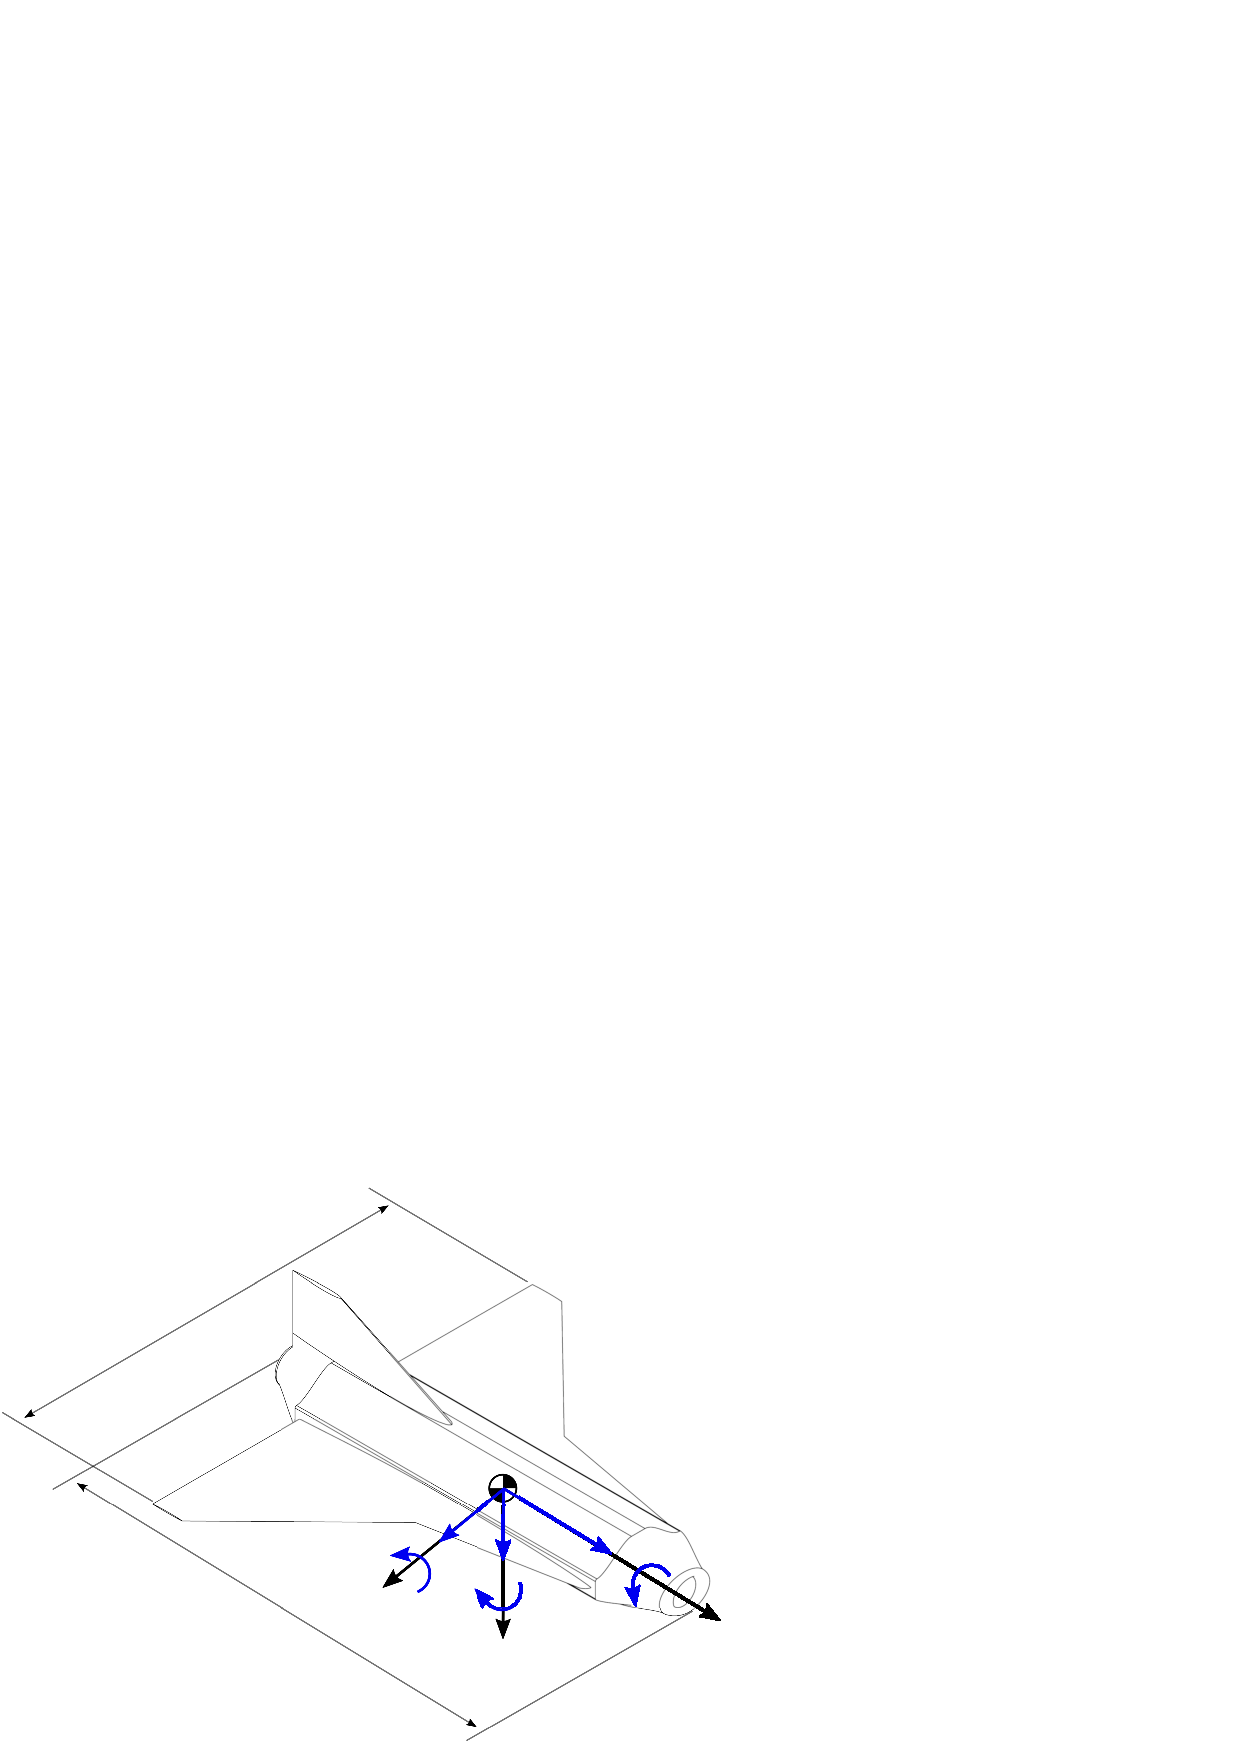
\includegraphics[width=0.7\textwidth]{Photos/MUFASA/MUFASA-ISO-Frames-BodyLength.png}
	\def\svgwidth{0.7\textwidth}
	\input{Photos/MUFASA/MUFASA-ISO-Frames-BodyLength.eps_tex}
	\caption{MUFASA B aerodynamic design and coordinate system.}
	\label{fig:mufasaB2}
	\hfill
\end{figure}

\noindent 
This type of figure is generated using the following commands: 

\begin{verbatim}
	\begin{figure}[hbt!]
		\centering
		\captionsetup{width=0.7\textwidth}
		%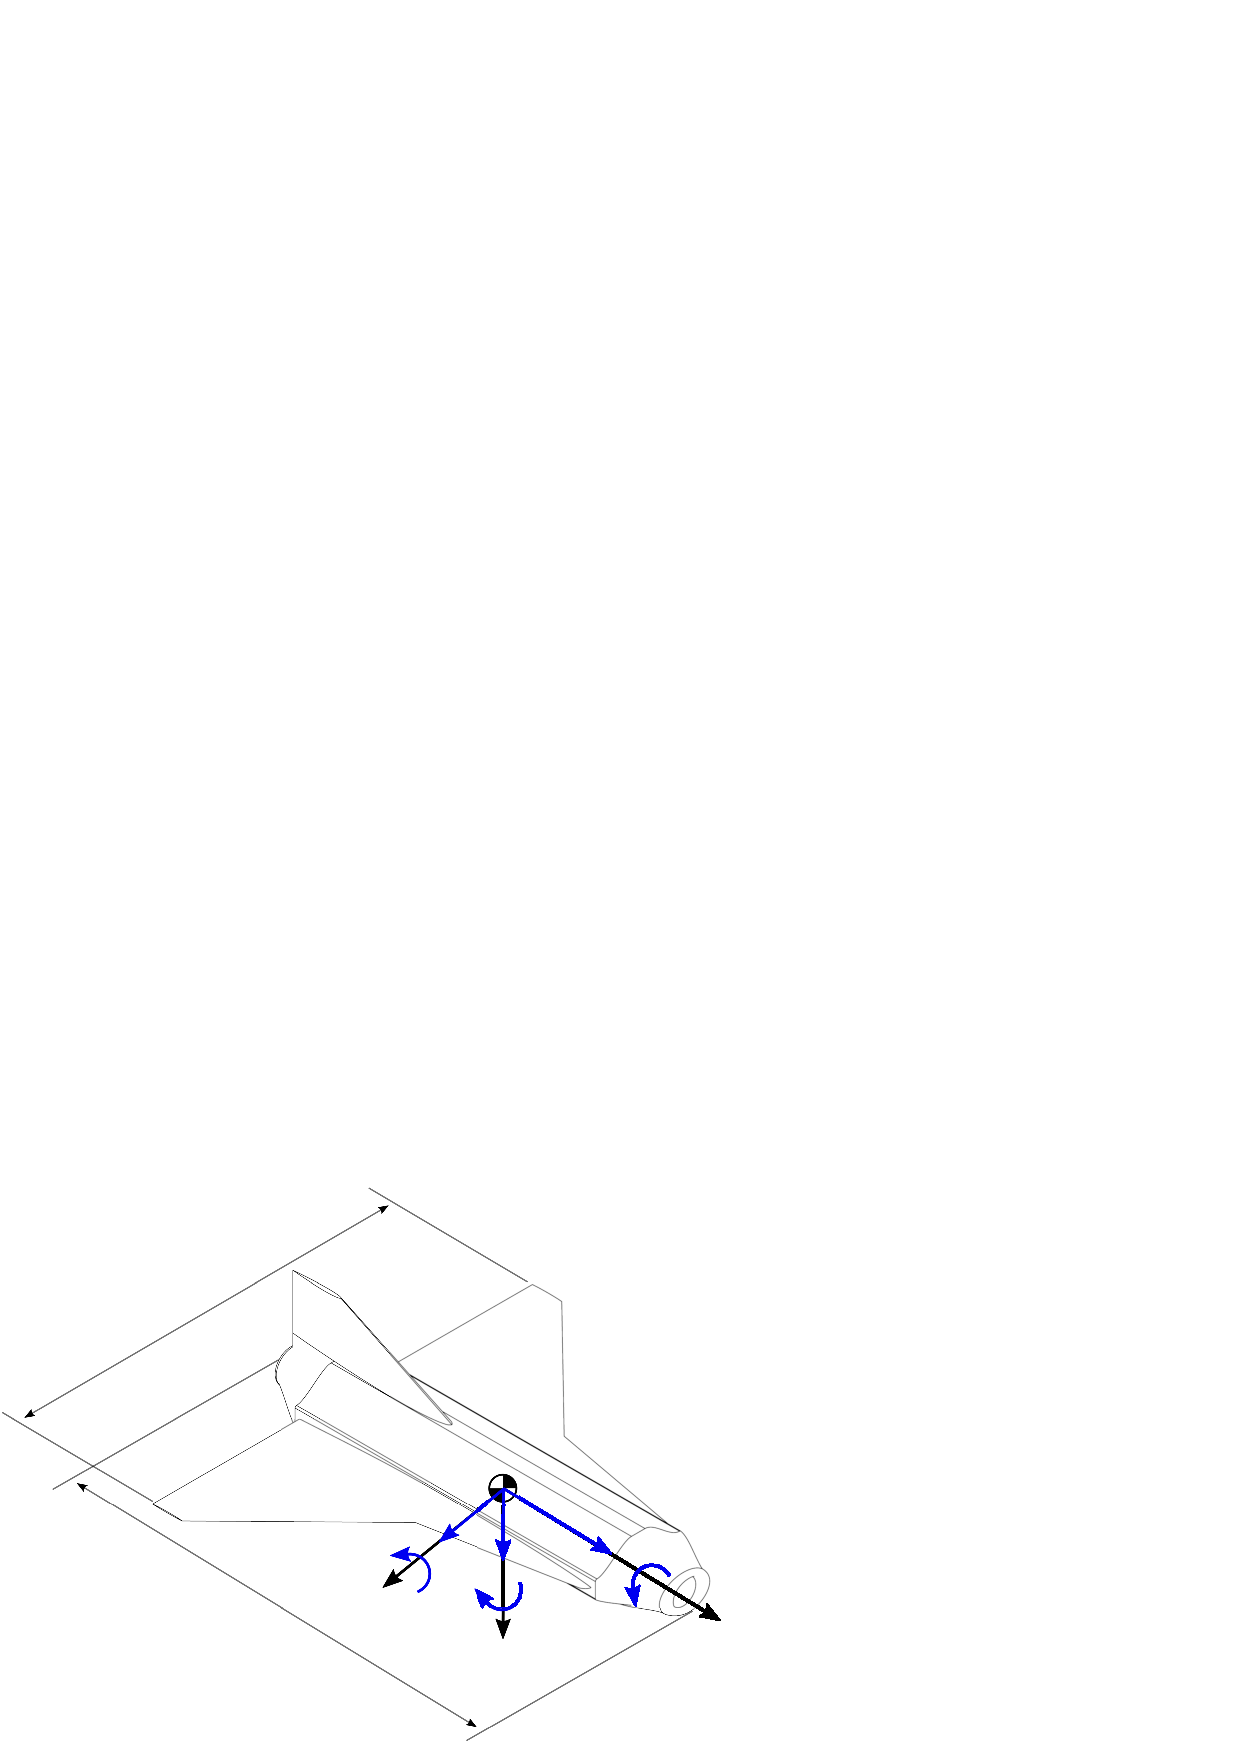
\includegraphics[width=0.7\textwidth]{Photos/MUFASA/MUFASA-ISO-Frames-BodyLength.png}
		\def\svgwidth{0.7\textwidth}
		\input{Photos/MUFASA/MUFASA-ISO-Frames-BodyLength.eps_tex}
		\caption{MUFASA B aerodynamic design and coordinate system.}
		\label{fig:mufasaB2}
		\hfill
	\end{figure}
\end{verbatim}

\subsection{Equations}
When coding an equation, carefully consider what is a variable and what is a label. 
Variables should be in math text, while labels should be in regular text. 
For example, in \cref{eqn:netForce}, $F_{\text{net}}$ is net force, not force as a function of variables $n \times e \times t$. 
Regular text can be inserted into an equation via the \verb*|\text{}| command. 

\begin{equation} \label{eqn:netForce}
	F_{\text{net}} = F_{\text{aero}} + F_{\text{g}} + F_{\text{T}}
\end{equation}


\subsection{Figure Creation}
\subsection{Custom Variable Creation}
\newcommand{\ap}{ArduPilot}
Local document variables are a way to aid in typing repetitive words or numerical values. 
These custom variables also aid in document consistency when referring to repeated words or values. 
An example of using locally defined document variables is creating a command to represent the word \textit{ArduPilot}. 
Due to the letters in \textit{ArduPilot}, it is an awkward word to type and a coding shorthand is created using the command: \verb*|\newcommand{\ap}{ArduPilot}|. 
Now, by typing \verb*|\ap\|, the word \ap\ is seamlessly inserted into the text. 
Note that the \verb*|\| following the \verb*|\ap| indicates a space should be left following the word \ap.

\LaTeX\ variables also work when inserted into InkScape generated figures, as outlined in the following YouTube video: \url{https://youtu.be/r0G44lxhTwc?si=SVSKCUj6mTy4rGCN}. 
Using variables in a diagram increases writing efficiency as it reduces the need to manually regenerate diagrams to change a variable when using the workflow presented in \Cref{sec:diagramCreation}. 
	%\section*{Appendix}

	%An Appendix, if needed, should appear before the acknowledgments.

	\section*{Acknowledgments}
	Funding for this work was provided by the AERO-CORE research group. 

	\bibliography{library_ben}

\end{document}
